\begin{figure}[H]
    \centering
    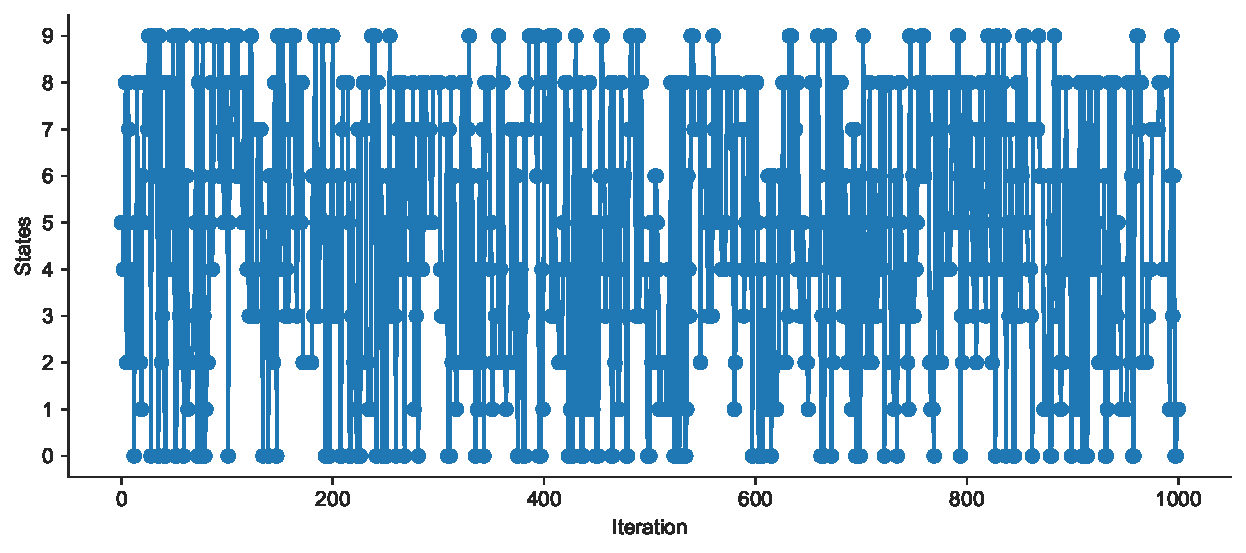
\includegraphics[width=0.8\linewidth]{data/05_reporting/problem_set_2/walk_plot.pdf}
    \caption{Example MCMC chain for $N=10$.}
    \label{fig:walk-plot}
\end{figure}

\begin{figure}[H]
    \centering
    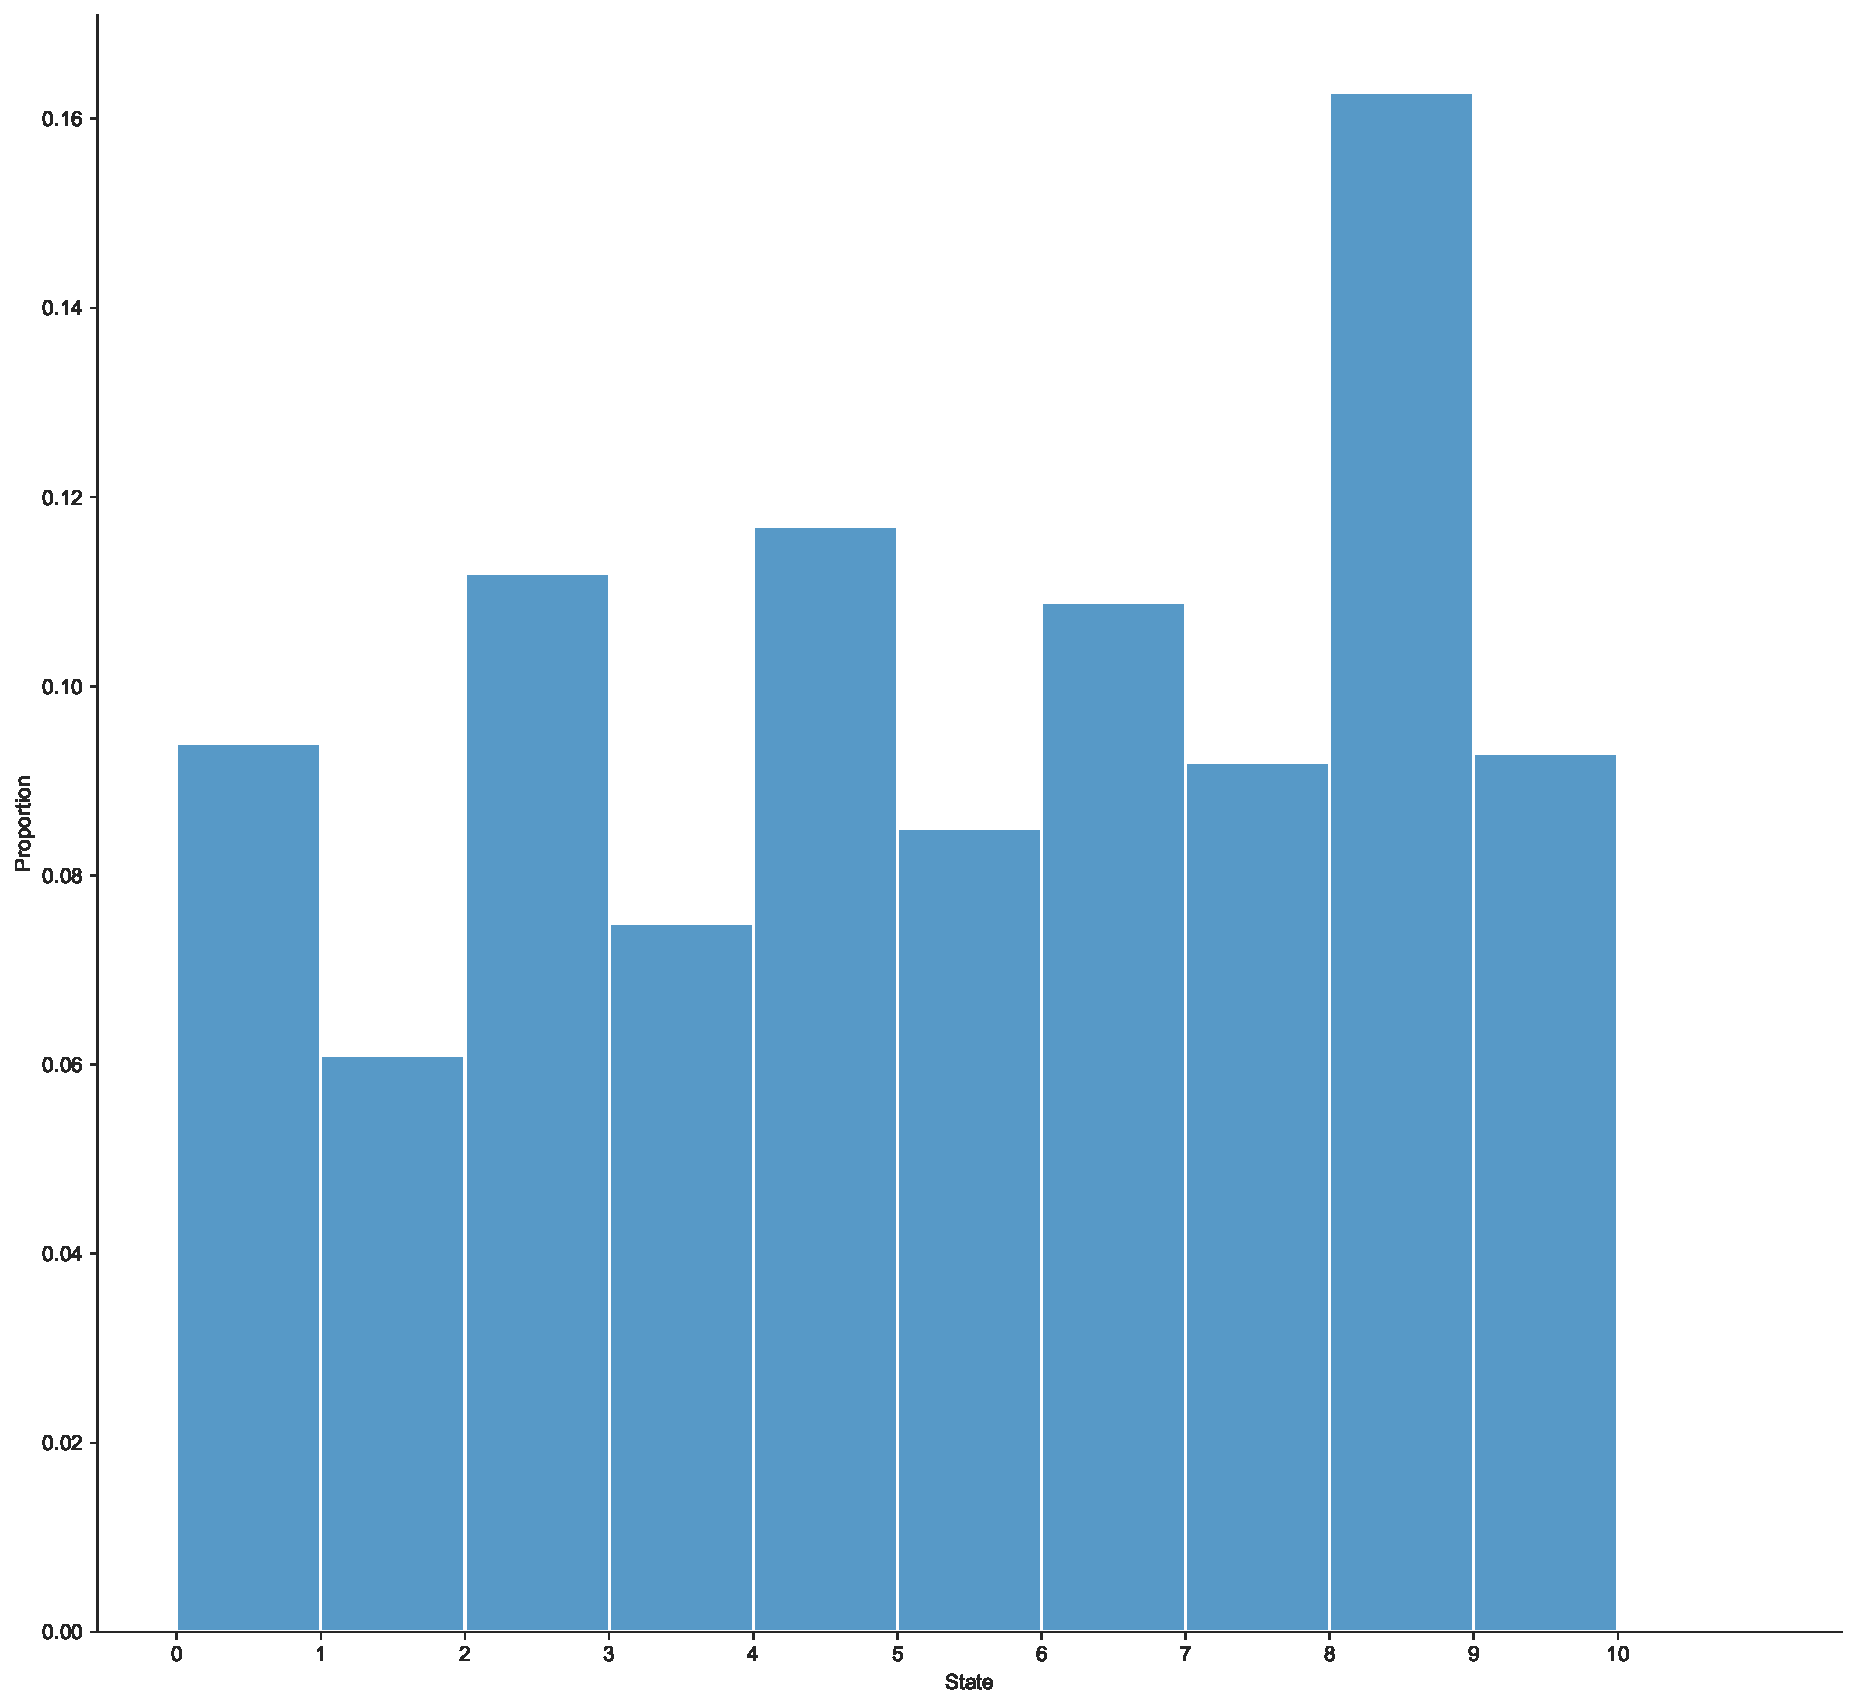
\includegraphics[width=\linewidth]{data/05_reporting/problem_set_2/state_probability.pdf}
    \caption{State probability distribution for $N=10$.}
    \label{fig:enter-label}
\end{figure}

\begin{figure}[H]
    \centering
    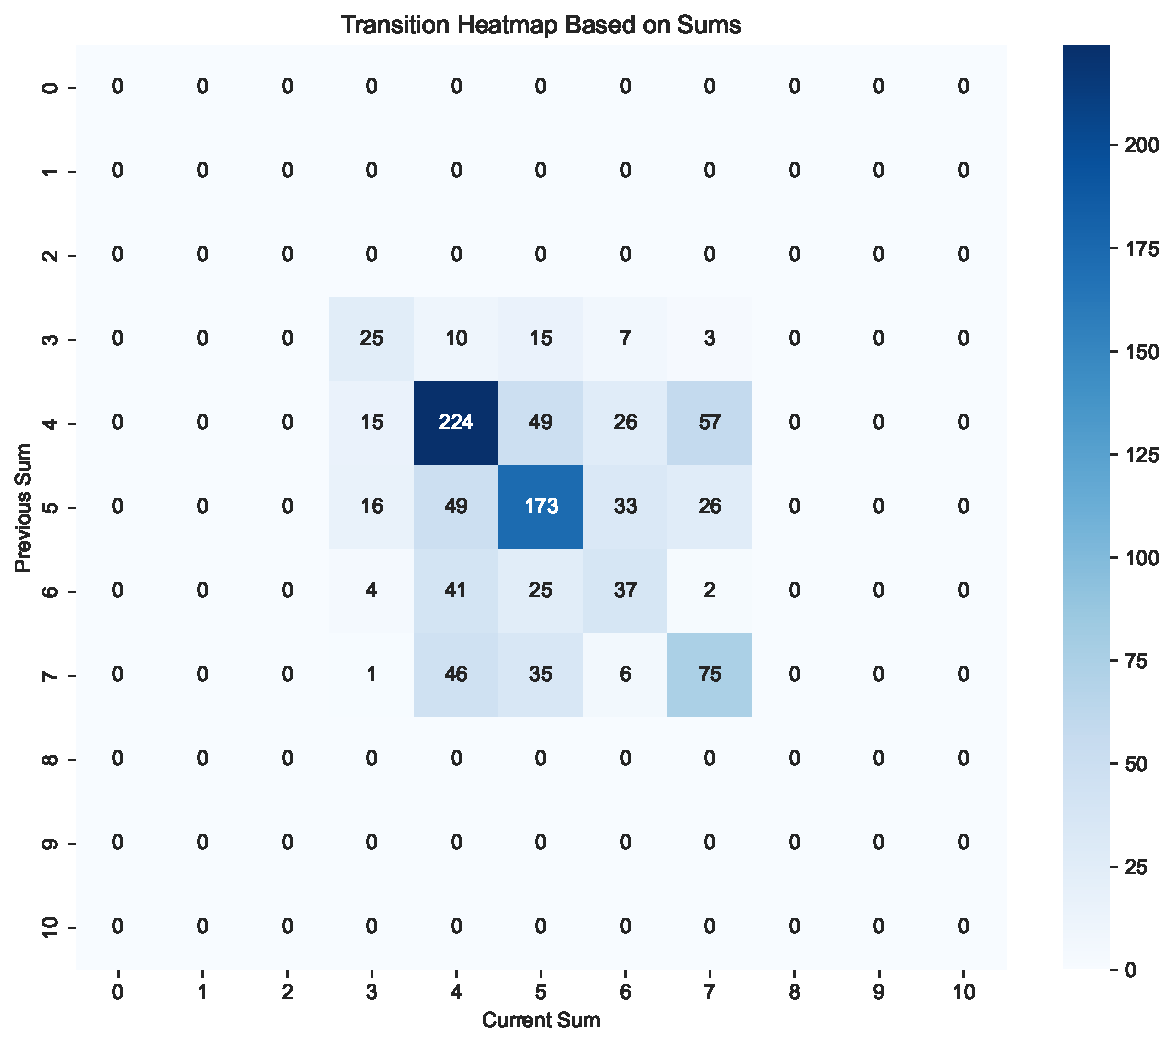
\includegraphics[width=\linewidth]{data/05_reporting/problem_set_2/transition_heatmap.pdf}
    \caption{State transition heat map. Each cell ($i, j$) represents the number of times the chain moved from a state with sum $i$ to a state with sum $j$.}
    \label{fig:enter-label}
\end{figure}